Below are the list of methods we will be using to solve the project goals.

\begin{itemize}

\item \textbf{Graph Representation}
\bigskip
In order to be able to predict the atomic scale fracture nucleation and propagation in silica-based glasses, we must first find an appropriate mathematical graph representation. 
\begin{itemize}
    \item \textbf{Basic Graph Representation}
    \\
    \\
    The most basic way to define a graph is naive. In one sample, we have a total number of $n$ atoms. An atom, either a Silicon atom or an Oxygen atom, is defined as a vertex $v_i$, where $0 \leq i \leq n$ and a set of such vertices is $\mathbf{V} = \{v_0,v_1,...v_{n-1}\}$. An edge, $e_i$ is defined as a mechanical trusses between two atoms. A set of such edges is $\mathbf{E} = \{e_0,e_1,...e_{n-1}\}$. As uni-axial stress is applied to the material, edges could break and form between any two vertices, where state 1 means an edge is broken and state 0 means an edge exists. Therefore, an set of active edges, defined as $\mathbf{E_a}$, includes all the edges that have broke or formed at least once, meaning they have changed their state, either from 1 to 0 or from 0 to 1 at one point. As a result, the graph $\mathbf{G}$ is thus defined as a discrete set of vertices $\mathbf{V}$ connected by a set of edges $\mathbf{E}$. We can denote it as $\ \mathbf{G} = (\mathbf{V},\mathbf{E})$, where the size of the graph is $\ |\mathbf{V}| = n $.
    \\
    \\
    Therefore, a simplified example of our constructed graph could result like this:
    \bigskip
    \\
    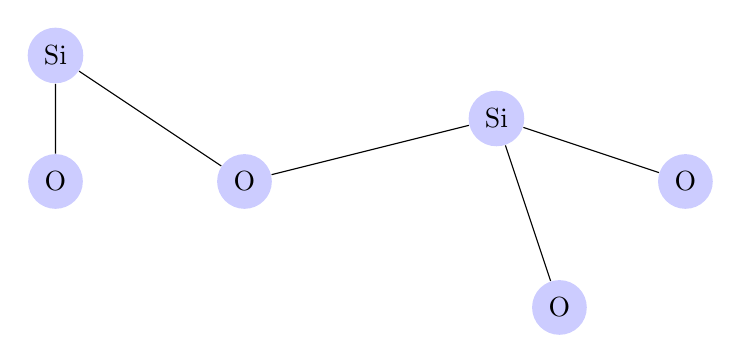
\begin{tikzpicture}
      [scale=.8,auto=left,every node/.style={circle,fill=blue!20}]
      \node (n6) at (1,10) {Si};
      \node (n4) at (4,8)  {O};
      \node (n5) at (8,9)  {Si};
      \node (n1) at (11,8) {O};
      \node (n2) at (9,6)  {O};
      \node (n7) at (1,8)  {O};
    
      \foreach \from/\to in {n6/n4,n4/n5,n5/n1,n2/n5,n6/n7}
        \draw (\from) -- (\to);
    
    \end{tikzpicture}
    \bigskip
    \\





    \item \textbf{Reduced Graph Representation}
    \\
    
    
\end{itemize}


\item \textbf{Feature Description}
\bigskip

To use ML algorithms, we want to characterize vertices based on features such as charge, stress tensor, type and centrality.

\begin{itemize}
    \item \textbf{Centrality:} In graph theory, centrality can be used to identify the most important vertices. An example could be a specific silicon atom that is at the center of where a fracture nucleates. Identifying these vertices with the most centrality will allow us to predict fracture nucleation.
    
    \bigskip
    
    More specifically, the vertex with the highest centrality degree would be surrounded by the most active bonds. Bonds that are not active do not necessarily contribute to the nucleation of a fracture. Thus, we can use vertices with high degrees of centrality to predict the location of fracture nucleation.
    
    \bigskip
    
    We want to observe degree centrality to examine both fracture nucleation and propagation. Centrality will give a number of connections to a vertex that will also allow us to examine 
    
    There are two types of degree centrality: in-degree and out-degree. In-degree gives a number of connections to a vertex and out-degree gives a number of connections that a vertex directs to other vertices. Both are significant to predicting fracture nucleation and propagation. We want to examine both in-degree and out-degree for all vertices. Vertices with greater in-degrees may directly contribute to fracture nucleation. Additionally, vertices with greater out-degrees may be used to predict the size of fracture propagation.
    
\end{itemize}







\\

\item \textbf{Machine Learning Methods}
\bigskip
\\
The culminating purpose of this project is to produce a machine learning model based on supervised learning techniques. Supervised learning is the results 

%Machine learning introduction. Talk about self driving cars people love that. 

%Speak about Regression and Classification methods. 

%Break up the data into training , validation , testing sets. 

%Regularization methods. LASSO , Ridge..


\begin{itemize}
\bigskip
\item \textbf{Method for Classifying Whether or not a vertex is part of a fracture}
\bigskip
\\
%Random forrest. Boosting, bagging. 


\item \textbf{Method for Predicting the Displacement of Vertices Dynamically}
\bigskip
\\

%RNN, LSTM, 

\end{itemize}


\end{itemize}